\documentclass[11pt,a4paper]{article}

\usepackage[utf8]{inputenc}
\usepackage[T1]{fontenc}
\usepackage{lmodern}
\usepackage[margin=2.2cm]{geometry}
\usepackage{amsmath,amssymb,mathtools,bm}
\usepackage{booktabs,tabularx,longtable,array}
\usepackage{enumitem}
\usepackage[raggedright]{titlesec}
\usepackage{xcolor}
\usepackage{hyperref}
\usepackage{tikz}
\usetikzlibrary{arrows.meta,positioning,fit,backgrounds,calc}

\hypersetup{
    colorlinks=true,
    linkcolor=blue!60!black,
    urlcolor=blue!60!black,
    citecolor=blue!60!black
}

\newcolumntype{L}[1]{>{\raggedright\arraybackslash}p{#1}}
\newcolumntype{C}[1]{>{\centering\arraybackslash}p{#1}}
\newcolumntype{Y}{>{\raggedright\arraybackslash}X}

\newcommand{\importantbox}[2]{%
  \par\medskip\noindent
  \fcolorbox{blue!50!black}{blue!4!white}{%
    \parbox{\dimexpr\linewidth-2\fboxsep-2\fboxrule\relax}{%
      \textbf{#1}\par\smallskip #2%
    }%
  }\par\medskip
}

\setlength{\parskip}{0.45em}
\setlength{\parindent}{0pt}

% Every section starts on a new page
\let\origsection\section
\renewcommand{\section}{\clearpage\origsection}

\title{\textbf{Atom-to-Reactor: Complete Mathematical \& Computational Model Reference}}
\author{Department of Chemistry -- \AA ngstr\"om Laboratory, Uppsala University}
\date{}

\begin{document}
\sloppy
\maketitle

This document provides a complete, equation-by-equation explanation of the \textbf{Atom-to-Reactor} multiscale framework implemented in the \texttt{kinetics/\allowbreak{}} package. It traces the full calculation pipeline from gas-phase Density Functional Theory (DFT) and Molecular Dynamics (MD) solvation energies to:

\begin{enumerate}[leftmargin=1.8em]
    \item \textbf{Equilibrium concentrations} $C_i^{\text{eq}}(T)$ via convex thermodynamic Gibbs free-energy minimization (\texttt{kinetics/\allowbreak{}thermo/\allowbreak{}equilibrium.py}),
    \item \textbf{Time-resolved concentration trajectories} $C_i(t)$ via transition-state theory, Marcus/BEP activation barrier laws, and stiff mass-action ODE integration (\texttt{kinetics/\allowbreak{}microkinetics/\allowbreak{}} and \texttt{kinetics/\allowbreak{}reactor/\allowbreak{}}), and
    \item \textbf{Experimental NMR observables} ($^{31}\text{P}$, $^{13}\text{C}$, $^{29}\text{Si}$, and $^1\text{H}$ window shares and millimolar concentrations) used in the thermodynamic and kinetic parameter fits (\texttt{kinetics/\allowbreak{}fitting/\allowbreak{}}).
\end{enumerate}


\section{High-Level Architecture}

\begin{center}
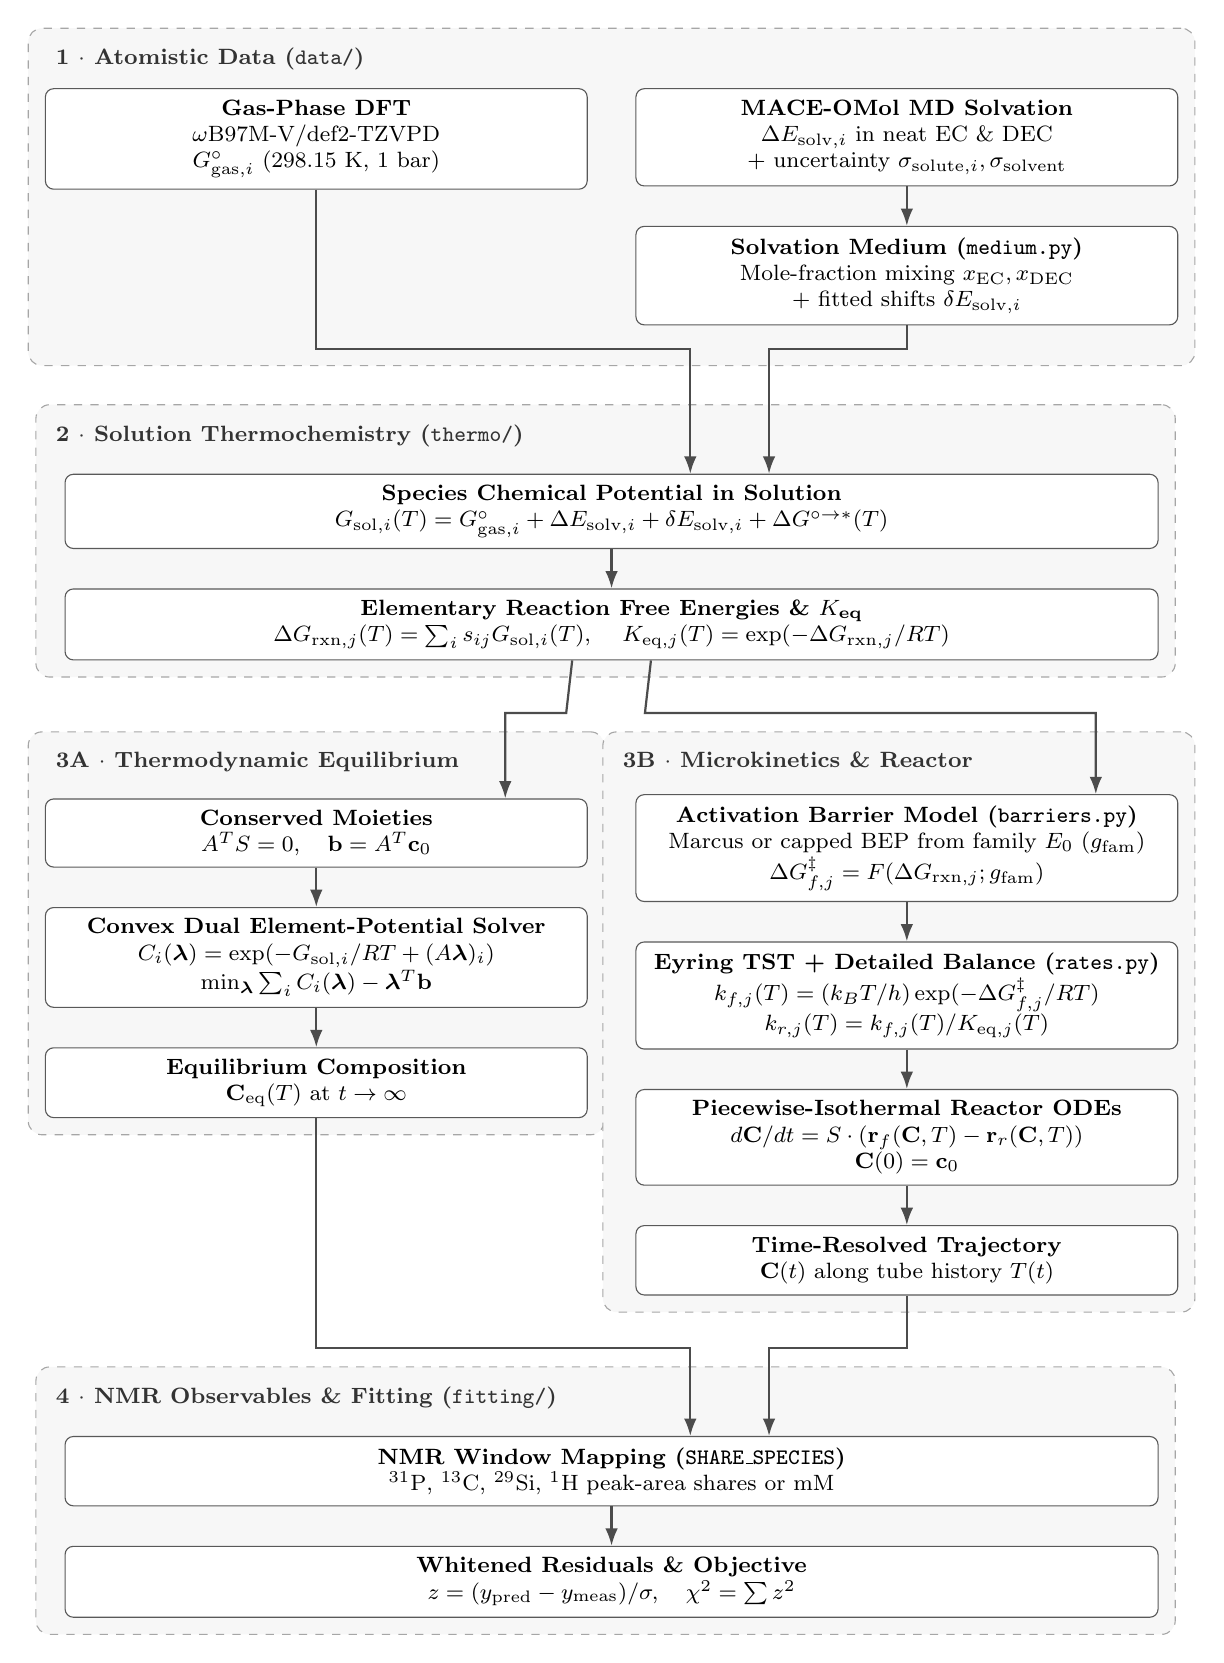
\begin{tikzpicture}[
    box/.style={draw=black!65, rounded corners=3pt, fill=white, align=flush center,
        font=\footnotesize, inner sep=4pt, text width=6.6cm, anchor=north},
    widebox/.style={box, text width=13.6cm},
    group/.style={draw=black!35, dashed, rounded corners=5pt, fill=black!3, inner sep=6pt},
    grouplabel/.style={font=\footnotesize\bfseries, text=black!80, anchor=north west, inner sep=1pt},
    arr/.style={-{Latex[length=2.2mm,width=1.6mm]}, thick, draw=black!70}
]
% x positions: left column -3.6, right column 3.6, wide boxes 0
% ---------------- Block 1
\node[grouplabel] (L1) at (-7.1,0) {1 $\cdot$ Atomistic Data (\texttt{data/\allowbreak{}})};
\node[box] (DFT) at (-3.75,-0.55) {\textbf{Gas-Phase DFT}\\$\omega$B97M-V/def2-TZVPD\\$G^\circ_{\text{gas},i}$ (298.15 K, 1 bar)};
\node[box] (MD)  at ( 3.75,-0.55) {\textbf{MACE-OMol MD Solvation}\\$\Delta E_{\text{solv},i}$ in neat EC \& DEC\\+ uncertainty $\sigma_{\text{solute},i}, \sigma_{\text{solvent}}$};
\node[box, below=0.5cm of MD.south, anchor=north] (MED) {\textbf{Solvation Medium (\texttt{medium.py})}\\Mole-fraction mixing $x_{\text{EC}}, x_{\text{DEC}}$\\+ fitted shifts $\delta E_{\text{solv},i}$};
\coordinate (J1) at ($(MED.south)+(0,-0.3)$);
\begin{scope}[on background layer]
  \node[group, fit=(L1)(DFT)(MD)(MED)(J1)] (B1) {};
\end{scope}
% ---------------- Block 2
\node[grouplabel] (L2) at ($(B1.south -| L1.west)+(0,-0.7)$) {2 $\cdot$ Solution Thermochemistry (\texttt{thermo/\allowbreak{}})};
\node[widebox] (GSOL) at ($(L2.south -| 0,0)+(0,-0.3)$) {\textbf{Species Chemical Potential in Solution}\\$G_{\text{sol},i}(T) = G^\circ_{\text{gas},i} + \Delta E_{\text{solv},i} + \delta E_{\text{solv},i} + \Delta G^{\circ\to *}(T)$};
\node[widebox, below=0.5cm of GSOL.south, anchor=north] (DGRXN) {\textbf{Elementary Reaction Free Energies \& $K_{\text{eq}}$}\\$\Delta G_{\text{rxn},j}(T) = \sum_i s_{ij} G_{\text{sol},i}(T)$, \quad $K_{\text{eq},j}(T) = \exp(-\Delta G_{\text{rxn},j} / RT)$};
\begin{scope}[on background layer]
  \node[group, fit=(L2)(GSOL)(DGRXN)] (B2) {};
\end{scope}
% ---------------- Block 3A and 3B
\node[grouplabel] (L3A) at ($(B2.south -| L1.west)+(0,-0.9)$) {3A $\cdot$ Thermodynamic Equilibrium};
\node[grouplabel] (L3B) at ($(B2.south -| 0.1,0)+(0,-0.9)$) {3B $\cdot$ Microkinetics \& Reactor};
\node[box] (CONSERV) at ($(L3A.south -| -3.75,0)+(0,-0.3)$) {\textbf{Conserved Moieties}\\$A^T S = 0, \quad \mathbf{b} = A^T \mathbf{c}_0$};
\node[box, below=0.5cm of CONSERV.south, anchor=north] (DUAL) {\textbf{Convex Dual Element-Potential Solver}\\$C_i(\bm{\lambda}) = \exp(-G_{\text{sol},i}/RT + (A\bm{\lambda})_i)$\\$\min_{\bm{\lambda}} \sum_i C_i(\bm{\lambda}) - \bm{\lambda}^T \mathbf{b}$};
\node[box, below=0.5cm of DUAL.south, anchor=north] (CEQ) {\textbf{Equilibrium Composition}\\$\mathbf{C}_{\text{eq}}(T)$ at $t \to \infty$};
\node[box] (BARR) at ($(L3B.south -| 3.75,0)+(0,-0.3)$) {\textbf{Activation Barrier Model (\texttt{barriers.py})}\\Marcus or capped BEP from family $E_0$ ($g_{\text{fam}}$)\\$\Delta G^\ddagger_{f,j} = F(\Delta G_{\text{rxn},j}; g_{\text{fam}})$};
\node[box, below=0.5cm of BARR.south, anchor=north] (RATES) {\textbf{Eyring TST + Detailed Balance (\texttt{rates.py})}\\$k_{f,j}(T) = (k_B T / h)\exp(-\Delta G^\ddagger_{f,j} / RT)$\\$k_{r,j}(T) = k_{f,j}(T) / K_{\text{eq},j}(T)$};
\node[box, below=0.5cm of RATES.south, anchor=north] (ODE) {\textbf{Piecewise-Isothermal Reactor ODEs}\\$d\mathbf{C}/dt = S\cdot(\mathbf{r}_f(\mathbf{C},T) - \mathbf{r}_r(\mathbf{C},T))$\\$\mathbf{C}(0) = \mathbf{c}_0$};
\node[box, below=0.5cm of ODE.south, anchor=north] (CT) {\textbf{Time-Resolved Trajectory}\\$\mathbf{C}(t)$ along tube history $T(t)$};
\begin{scope}[on background layer]
  \node[group, fit=(L3A)(CONSERV)(DUAL)(CEQ)] (B3A) {};
  \node[group, fit=(L3B)(BARR)(RATES)(ODE)(CT)] (B3B) {};
\end{scope}
% ---------------- Block 4
\coordinate (J4) at ($(B3B.south)+(0,-0.45)$);
\node[grouplabel] (L4) at ($(J4 -| L1.west)+(0,-0.45)$) {4 $\cdot$ NMR Observables \& Fitting (\texttt{fitting/\allowbreak{}})};
\node[widebox] (NMR) at ($(L4.south -| 0,0)+(0,-0.3)$) {\textbf{NMR Window Mapping (\texttt{SHARE\_\allowbreak{}SPECIES})}\\$^{31}\text{P}$, $^{13}\text{C}$, $^{29}\text{Si}$, $^1\text{H}$ peak-area shares or mM};
\node[widebox, below=0.5cm of NMR.south, anchor=north] (CHI2) {\textbf{Whitened Residuals \& Objective}\\$z = (y_{\text{pred}} - y_{\text{meas}}) / \sigma, \quad \chi^2 = \sum z^2$};
\begin{scope}[on background layer]
  \node[group, fit=(L4)(NMR)(CHI2)] (B4) {};
\end{scope}
% ---------------- Arrows (vertical legs kept clear of the group labels)
\draw[arr] (DFT.south) -- (DFT.south |- J1) -| ($(GSOL.north)+(1.0,0)$);
\draw[arr] (MD.south) -- (MED.north);
\draw[arr] (MED.south) -- (MED.south |- J1) -| ($(GSOL.north)+(2.0,0)$);
\draw[arr] (GSOL.south) -- (DGRXN.north);
\coordinate (J3) at ($(B2.south)+(0,-0.45)$);
\draw[arr] ($(DGRXN.south)+(-0.5,0)$) -- ($(J3)+(-0.5,0)$) -| ($(CONSERV.north)+(2.4,0)$);
\draw[arr] ($(DGRXN.south)+(0.5,0)$) -- ($(J3)+(0.5,0)$) -| ($(BARR.north)+(2.4,0)$);
\draw[arr] (CONSERV.south) -- (DUAL.north);
\draw[arr] (DUAL.south) -- (CEQ.north);
\draw[arr] (BARR.south) -- (RATES.north);
\draw[arr] (RATES.south) -- (ODE.north);
\draw[arr] (ODE.south) -- (CT.north);
\draw[arr] (CEQ.south) -- (CEQ.south |- J4) -| ($(NMR.north)+(1.0,0)$);
\draw[arr] (CT.south) -- (CT.south |- J4) -| ($(NMR.north)+(2.0,0)$);
\draw[arr] (NMR.south) -- (CHI2.north);
\end{tikzpicture}
\end{center}

\clearpage
\subsection*{Codebase Map by Module}

Paths are relative to the \texttt{kinetics/\allowbreak{}} package.

\begin{tabularx}{\textwidth}{L{4.9cm} Y}
\toprule
\textbf{Package / Module} & \textbf{Role in the Mathematical Pipeline} \\
\midrule
\texttt{constants.py} & CODATA 2018 fundamental constants ($R, k_B, h, N_A$), standard states ($P^\circ = 1\text{ bar}, c^* = 1\text{ M}$), and unit conversions ($\text{E}_{\text{h}} \to \text{eV} \to \text{kJ/mol}$). \\[3pt]
\texttt{data/\allowbreak{}species.py} & Loads gas-phase DFT energies (\texttt{G\_\allowbreak{}gas\_\allowbreak{}eV}, \texttt{H\_\allowbreak{}gas\_\allowbreak{}eV}, \texttt{E\_\allowbreak{}scf\_\allowbreak{}eV}) and MD solvation energies (\texttt{dE\_\allowbreak{}solv\_\allowbreak{}eV}, \texttt{dE\_\allowbreak{}solv\_\allowbreak{}sigma\_\allowbreak{}eV}) from the Tank snapshot. \\[3pt]
\texttt{data/\allowbreak{}medium.py} & Defines \texttt{SolvationMedium}, converting solvent volume fractions into mole fractions $x_s$ and combining neat MD solvation energies. \\[3pt]
\texttt{data/\allowbreak{}network.py} & Defines the elementary reaction network (\texttt{R1}--\texttt{R9} and optional \texttt{N10}--\texttt{N15}), tracked species, stoichiometric matrix $S$, and mass-action order matrices. \\[3pt]
\texttt{thermo/\allowbreak{}gas.py} & Gas-phase thermochemistry: stored RRHO Gibbs energy at $298.15\text{ K}$ (\texttt{wb97mv}) or Grimme quasi-RRHO statistical mechanics (\texttt{qRRHO}). \\[3pt]
\texttt{thermo/\allowbreak{}standard\_\allowbreak{}state.py} & Standard-state compression shift $\Delta G^{\circ \to *}(T)$ from $1\text{ bar}$ ideal gas to $1\text{ mol/L}$ solution. \\[3pt]
\texttt{thermo/\allowbreak{}solution.py} & Solution-phase Gibbs free energy $G_{\text{sol}, i}(T)$ (\texttt{calculate\_\allowbreak{}solution\_\allowbreak{}gibbs}). \\[3pt]
\texttt{thermo/\allowbreak{}reaction.py} & Reaction free energies $\Delta G_{\text{rxn}, j}(T)$ and equilibrium constants $K_{\text{eq}, j}(T)$ (\texttt{calculate\_\allowbreak{}reaction\_\allowbreak{}thermo}). \\[3pt]
\texttt{thermo/\allowbreak{}uncertainty.py} & Propagates solute and shared pure-solvent MD uncertainties into reaction covariance $\Sigma$ and maps reaction shifts to species shifts. \\[3pt]
\texttt{thermo/\allowbreak{}equilibrium.py} & Algebraic closed-tube equilibrium solver via convex dual element potentials (\texttt{calculate\_\allowbreak{}equilibrium}). \\[3pt]
\texttt{microkinetics/\allowbreak{}barriers.py} & Maps $\Delta G_{\text{rxn}, j}$ and family intrinsic barrier $g$ ($E_0$) to forward activation barrier $\Delta G_{f,j}^\ddagger$ (\texttt{marcus}, \texttt{bep\_\allowbreak{}cap}). \\[3pt]
\texttt{microkinetics/\allowbreak{}rates.py} & Eyring transition-state theory for $k_{f,j}(T)$, optional Collins--Kimball diffusion ceiling $k_D$, and detailed balance $k_{r,j}(T) = k_{f,j}(T)/K_{\text{eq}, j}(T)$. \\[3pt]
\texttt{reactor/\allowbreak{}engine.py} & \texttt{MassActionSystem}: net reaction rates $\mathbf{r}(\mathbf{C})$, ODE right-hand side $\frac{d\mathbf{C}}{dt} = S\,\mathbf{r}$, exact analytical Jacobian, and stiff ODE integration (\texttt{Radau}/\texttt{BDF}). \\[3pt]
\texttt{reactor/\allowbreak{}protocol.py} & Piecewise-isothermal multi-stage integration along experimental sample histories (\texttt{simulate\_\allowbreak{}history}, \texttt{simulate\_\allowbreak{}protocol}). \\[3pt]
\texttt{fitting/\allowbreak{}residuals.py} & Maps simulated concentrations to NMR window shares (\texttt{SHARE\_\allowbreak{}SPECIES}), applies the noise/baseline/floor error model, and computes whitened residuals. \\[3pt]
\texttt{fitting/\allowbreak{}thermo\_\allowbreak{}fit.py} & \texttt{ThermoProblem}: equilibrium spectrum selection, replicate compatibility, and fitting species solvation shifts $\delta E_{\text{solv}, i}$ to equilibrium NMR data. \\[3pt]
\texttt{fitting/\allowbreak{}candidates.py} \& \texttt{estimation.py} & \texttt{FitStructure} and \texttt{FitProblem}: kinetic candidate structures (\texttt{M0}, \texttt{M1}, \texttt{M1-split}, \texttt{M3-split}), Sobol + TRF optimization, and profile likelihoods. \\
\bottomrule
\end{tabularx}


\section{Chemical System \& Reaction Network (\texttt{kinetics/\allowbreak{}data/\allowbreak{}network.py})}

\subsection{Tracked Species}

When tris(trimethylsilyl) phosphate (\textbf{TMSPA}, $\text{OP(OSiMe}_3)_3$) scavenges trace water in a carbonate electrolyte (ethylene carbonate \textbf{EC} or an \textbf{EC:DEC} mixture), it undergoes a cascade of hydrolysis, silanol condensation, trans-silylation, and solvent ring-opening steps. The network tracks $N_{\text{sp}} = 11$ reactive species (\texttt{NETWORK\_\allowbreak{}SPECIES}):

\begin{tabularx}{\textwidth}{L{3.3cm} L{1.7cm} Y C{1.4cm} C{1.4cm}}
\toprule
\textbf{Group} & \textbf{Species ID} & \textbf{Chemical Formula / Identity} & \textbf{Silyl groups} & \textbf{P atoms} \\
\midrule
\textbf{Phosphate ester ladder} & \texttt{TMSPA} & $\text{OP(OSiMe}_3)_3$ --- tris(trimethylsilyl) phosphate & 3 & 1 \\
 & \texttt{BMSPA} & $\text{OP(OH)(OSiMe}_3)_2$ --- bis(trimethylsilyl) mono-acid phosphate & 2 & 1 \\
 & \texttt{MMSPA} & $\text{OP(OH)}_2(\text{OSiMe}_3)$ --- mono(trimethylsilyl) di-acid phosphate & 1 & 1 \\
 & \texttt{H3PO4} & $\text{OP(OH)}_3$ --- orthophosphoric acid & 0 & 1 \\
\midrule
\textbf{Water \& free silyl species} & \texttt{H2O} & $\text{H}_2\text{O}$ --- water & 0 & 0 \\
 & \texttt{TMSOH} & $\text{Me}_3\text{SiOH}$ --- trimethylsilanol & 1 & 0 \\
 & \texttt{HMDSO} & $\text{Me}_3\text{SiOSiMe}_3$ --- hexamethyldisiloxane & 2 & 0 \\
\midrule
\textbf{Solvent \& ring-opening products} & \texttt{EC} & $(\text{CH}_2\text{O})_2\text{CO}$ --- ethylene carbonate (solvent) & 0 & 0 \\
 & \texttt{TMSOEG} & $\text{Me}_3\text{SiOCH}_2\text{CH}_2\text{OH}$ --- 2-(trimethylsiloxy)ethanol & 1 & 0 \\
 & \texttt{TMSOdiEG} & $\text{Me}_3\text{SiOCH}_2\text{CH}_2\text{OSiMe}_3$ --- 1,2-bis(trimethylsiloxy)ethane & 2 & 0 \\
 & \texttt{CO2} & $\text{CO}_2$ --- carbon dioxide & 0 & 0 \\
\bottomrule
\end{tabularx}

\medskip
\emph{(Note: Diethyl carbonate \textbf{DEC} in 1:1 EC:DEC mixtures is chemically inert in this network and acts as a co-solvent that modifies the solvation medium and dilutes initial molarities.)}

\clearpage
\subsection{Elementary Reactions (\texttt{R1}--\texttt{R9} and \texttt{N10}--\texttt{N15})}

The default reaction network (\texttt{NETWORK} in \texttt{kinetics/\allowbreak{}data/\allowbreak{}network.py}) comprises 9 elementary reversible steps grouped into 4 reaction families:

\begin{tabularx}{\textwidth}{L{1.0cm} Y L{3.0cm} L{4.2cm}}
\toprule
\textbf{ID} & \textbf{Elementary Reaction} & \textbf{Reaction Family (\texttt{class})} & \textbf{Linear Dependency / Cycle Relation} \\
\midrule
\textbf{R1} & $\text{TMSPA} + \text{H}_2\text{O} \rightleftharpoons \text{BMSPA} + \text{TMSOH}$ & \texttt{hydrolysis} & Independent basis reaction \\
\textbf{R2} & $\text{BMSPA} + \text{H}_2\text{O} \rightleftharpoons \text{MMSPA} + \text{TMSOH}$ & \texttt{hydrolysis} & Independent basis reaction \\
\textbf{R3} & $\text{MMSPA} + \text{H}_2\text{O} \rightleftharpoons \text{H}_3\text{PO}_4 + \text{TMSOH}$ & \texttt{hydrolysis} & Independent basis reaction \\
\textbf{R4} & $2\,\text{TMSOH} \rightleftharpoons \text{HMDSO} + \text{H}_2\text{O}$ & \texttt{condensation} & Independent basis reaction \\
\textbf{R5} & $\text{TMSPA} + \text{TMSOH} \rightleftharpoons \text{BMSPA} + \text{HMDSO}$ & \texttt{transfer} & $\text{R5} = \text{R1} + \text{R4}$ \\
\textbf{R6} & $\text{BMSPA} + \text{TMSOH} \rightleftharpoons \text{MMSPA} + \text{HMDSO}$ & \texttt{transfer} & $\text{R6} = \text{R2} + \text{R4}$ \\
\textbf{R7} & $\text{MMSPA} + \text{TMSOH} \rightleftharpoons \text{H}_3\text{PO}_4 + \text{HMDSO}$ & \texttt{transfer} & $\text{R7} = \text{R3} + \text{R4}$ \\
\textbf{R8} & $\text{EC} + \text{TMSOH} \rightleftharpoons \text{TMSOEG} + \text{CO}_2$ & \texttt{solvent\_\allowbreak{}attack} & Independent basis reaction \\
\textbf{R9} & $\text{EC} + \text{TMSOEG} \rightleftharpoons \text{TMSOdiEG} + \text{CO}_2$ & \texttt{solvent\_\allowbreak{}attack} & Independent basis reaction \\
\bottomrule
\end{tabularx}

\medskip
In the extended network variants (\texttt{'R1-R9+N10-N15'} and \texttt{'R1-R9+N10-N15,\allowbreak{} fixed 1.15 eV'}), 6 additional reactions (\texttt{EXTRA\_\allowbreak{}REACTIONS}) between the same 11 species are included:
\begin{itemize}[leftmargin=1.8em]
    \item \textbf{N10} ($\text{exchange}$): $2\,\text{BMSPA} \rightleftharpoons \text{MMSPA} + \text{TMSPA}$ ($\text{N10} = \text{R2} - \text{R1}$)
    \item \textbf{N11} ($\text{exchange}$): $2\,\text{TMSOEG} \rightleftharpoons \text{TMSOH} + \text{TMSOdiEG}$ ($\text{N11} = \text{R9} - \text{R8}$, when coupled with $\text{R4}$)
    \item \textbf{N12} ($\text{hydrolysis}$, follows $\text{R2}$): $\text{BMSPA} + \text{H}_2\text{O} \rightleftharpoons \text{H}_3\text{PO}_4 + \text{HMDSO}$ ($\text{N12} = \text{R2} + \text{R7}$)
    \item \textbf{N13} ($\text{exchange}$): $\text{BMSPA} + \text{H}_3\text{PO}_4 \rightleftharpoons 2\,\text{MMSPA}$ ($\text{N13} = \text{R2} - \text{R3}$)
    \item \textbf{N14} ($\text{exchange}$): $\text{BMSPA} + \text{MMSPA} \rightleftharpoons \text{H}_3\text{PO}_4 + \text{TMSPA}$ ($\text{N14} = \text{R3} - \text{R1}$)
    \item \textbf{N15} ($\text{hydrolysis}$, follows $\text{R1}$): $\text{TMSPA} + \text{H}_2\text{O} \rightleftharpoons \text{MMSPA} + \text{HMDSO}$ ($\text{N15} = \text{R1} + \text{R6}$)
\end{itemize}

\subsection{Stoichiometric Matrix $S$ and Reaction Order Matrices}

For a network of $N_{\text{sp}}$ species and $N_{\text{rxn}}$ reactions, \texttt{build\_\allowbreak{}stoichiometric\_\allowbreak{}matrix} constructs the matrix $S \in \mathbb{R}^{N_{\text{sp}} \times N_{\text{rxn}}}$ with entries:
\begin{equation}
s_{i,j} = \nu_{i,j}^{\text{prod}} - \nu_{i,j}^{\text{react}}
\end{equation}
where $\nu_{i,j}^{\text{react}} \ge 0$ and $\nu_{i,j}^{\text{prod}} \ge 0$ are the forward and reverse molecularities returned by \texttt{build\_\allowbreak{}order\_\allowbreak{}matrices}.


\section{From Atomistic Energies (DFT \& MD) to Reaction Thermodynamics (\texttt{kinetics/\allowbreak{}thermo/\allowbreak{}})}

Both the thermodynamic equilibrium solver and the microkinetic ODE solver start from the exact same species chemical potentials in solution $G_{\text{sol}, i}(T)$ and elementary reaction free energies $\Delta G_{\text{rxn}, j}(T)$.

\subsection*{Step 3.1 $\cdot$ Gas-Phase DFT Gibbs Energy (\texttt{kinetics/\allowbreak{}thermo/\allowbreak{}gas.py})}

For each species $i$, the Tank dataset snapshot stores gas-phase DFT calculations at the \textbf{$\omega\text{B97M-V/def2-TZVPD}$} level of theory ($T_{\text{std}} = 298.15\text{ K}$, $P^\circ = 1\text{ bar} = 10^5\text{ Pa}$). Two thermochemical modes (\texttt{thermo\_\allowbreak{}mode}) are supported in \texttt{calculate\_\allowbreak{}gas\_\allowbreak{}thermo}:

\begin{enumerate}[leftmargin=1.8em]
    \item \textbf{\texttt{'wb97mv'} (Default across fits):} Uses the stored rigid-rotor harmonic-oscillator (RRHO) Gibbs free energy converted from Hartree to eV and kJ/mol ($1\text{ E}_{\text{h}} = 27.211386\text{ eV}$, $1\text{ eV} = 96.485332\text{ kJ/mol}$):
    \begin{equation}
    G_{\text{gas}, i}^\circ = E_{\text{gas}, i}^{\text{Eh}} \times 27.211386\text{ eV/E}_{\text{h}}
    \end{equation}
    \item \textbf{\texttt{'qRRHO'} (Grimme quasi-RRHO):} When vibrational frequencies $\{\tilde{\nu}_m\}$ and principal moments of inertia are present, computes translational (Sackur--Tetrode at $P^\circ = 1\text{ bar}$), rigid-rotor rotational, and damped quasi-RRHO vibrational enthalpies and entropies at temperature $T$ with damping frequency $\tilde{\nu}_0 = 100\text{ cm}^{-1}$:
    \begin{equation}
    w(\tilde{\nu}_m) = \frac{1}{1 + (\tilde{\nu}_0 / \tilde{\nu}_m)^4}, \qquad S_{\text{vib}} = \sum_m \left[ w(\tilde{\nu}_m) S_{\text{HO}}(\tilde{\nu}_m, T) + \big(1 - w(\tilde{\nu}_m)\big) S_{\text{free-rot}}(\tilde{\nu}_m, T) \right]
    \end{equation}
\end{enumerate}

\subsection*{Step 3.2 $\cdot$ Solvation Energy in Neat or Mixed Solvents (\texttt{kinetics/\allowbreak{}data/\allowbreak{}medium.py})}

Molecular dynamics (MD) simulations using the MACE-OMol machine-learned interatomic potential provide the solvation energy $\Delta E_{\text{solv}, i}^{(s)}$ of each solute $i$ in neat solvent $s \in \{\text{EC}, \text{DEC}\}$.

For a solvent mixture specified by volume fractions $\{f_s\}$ (such as \textbf{EC:DEC 1:1 by volume} in the lab NMR tubes), \texttt{SolvationMedium.mole\_\allowbreak{}fractions} converts volume fractions into mole fractions $x_s$ using the neat liquid densities ($\rho_{\text{EC}} = 1.321\text{ g/mL}$, $\rho_{\text{DEC}} = 0.975\text{ g/mL}$) and molar masses $M_s$:
\begin{equation}
n_s = \frac{f_s \, \rho_s}{M_s}, \qquad x_s = \frac{n_s}{\sum_{s'} n_{s'}} \qquad \big(\text{for EC:DEC 1:1 v/v: } x_{\text{EC}} \approx 0.645,\; x_{\text{DEC}} \approx 0.355\big)
\end{equation}

Under the linear ideal-mixing rule (\texttt{\_\allowbreak{}cached\_\allowbreak{}medium\_\allowbreak{}database}), the raw solvation energy of species $i$ in the mixture is the mole-fraction-weighted sum:
\begin{equation}
\Delta E_{\text{solv}, i}^{\text{raw}} = \sum_{s} x_s \, \Delta E_{\text{solv}, i}^{(s)}
\end{equation}

When species free-energy shifts $\delta E_{\text{solv}, i}$ are introduced (either during a thermodynamic fit in \texttt{thermo\_\allowbreak{}fit.py} or via freed reaction energies in \texttt{candidates.py}), the effective solvation energy becomes:
\begin{equation}
\Delta E_{\text{solv}, i} = \Delta E_{\text{solv}, i}^{\text{raw}} + \delta E_{\text{solv}, i}
\end{equation}

\subsection*{Step 3.3 $\cdot$ Standard-State Compression Shift (\texttt{kinetics/\allowbreak{}thermo/\allowbreak{}standard\_\allowbreak{}state.py})}

Gas-phase DFT quantities are referenced to an ideal gas at $P^\circ = 1\text{ bar}$ with molar concentration $c_{\text{gas}}^\circ(T) = \frac{P^\circ}{RT}$, whereas solution-phase thermodynamics and mass-action kinetics use a $c^* = 1\text{ mol/L} = 1000\text{ mol/m}^3$ reference state. Compressing 1 mole of ideal gas into 1 L of solution adds the entropic concentration shift (\texttt{calculate\_\allowbreak{}standard\_\allowbreak{}state\_\allowbreak{}shift}):
\begin{equation}
\Delta G^{\circ \to *}(T) = R T \ln\!\left(\frac{c^*}{P^\circ / (R T)}\right) = R T \ln\!\left(\frac{R T c^*}{P^\circ}\right) \qquad \big(+7.96\text{ kJ/mol} = +0.0825\text{ eV at } 298.15\text{ K}\big)
\end{equation}

\emph{(In \texttt{'wb97mv'} mode, $\Delta G^{\circ \to *}(T)$ is omitted from individual species energies because every reaction in the default network \texttt{R1}--\texttt{R9} and \texttt{N10}--\texttt{N15} is a $2 \to 2$ bimolecular step with $\Delta \nu_j = \sum_i s_{i,j} = 0$, so $\Delta G^{\circ \to *}(T)$ cancels out identically in every $\Delta G_{\text{rxn}, j}$.)}

\subsection*{Step 3.4 $\cdot$ Solution-Phase Chemical Potential $G_{\text{sol}, i}(T)$ (\texttt{kinetics/\allowbreak{}thermo/\allowbreak{}solution.py})}

Combining the gas-phase Gibbs energy, the solvation energy (plus any fitted shift $\delta E_{\text{solv}, i}$), and the standard-state shift yields the standard-state Gibbs energy (standard chemical potential $\mu_i^\circ(T)$) of species $i$ in solution (\texttt{calculate\_\allowbreak{}solution\_\allowbreak{}gibbs}):
\begin{equation}
\mu_i^\circ(T) \equiv G_{\text{sol}, i}(T) = G_{\text{gas}, i}^\circ(T) + \Delta E_{\text{solv}, i}^{\text{raw}} + \delta E_{\text{solv}, i} + \Delta G^{\circ \to *}(T)
\end{equation}

\subsection*{Step 3.5 $\cdot$ Elementary Reaction Free Energy $\Delta G_{\text{rxn}, j}(T)$ and Equilibrium Constant $K_{\text{eq}, j}(T)$ (\texttt{kinetics/\allowbreak{}thermo/\allowbreak{}reaction.py})}

For each elementary reaction $j$, \texttt{calculate\_\allowbreak{}reaction\_\allowbreak{}thermo} evaluates the standard reaction Gibbs free energy by multiplying $G_{\text{sol}, i}(T)$ by the stoichiometric coefficients $s_{i,j} = \nu_{i,j}^{\text{prod}} - \nu_{i,j}^{\text{react}}$:
\begin{equation}
\Delta G_{\text{rxn}, j}(T) = \sum_{i=1}^{N_{\text{sp}}} s_{i,j} \, G_{\text{sol}, i}(T) = \big(S^T \mathbf{G}_{\text{sol}}(T)\big)_j
\end{equation}

From $\Delta G_{\text{rxn}, j}(T)$, the dimensionless thermodynamic equilibrium constant at temperature $T$ is:
\begin{equation}
K_{\text{eq}, j}(T) = \exp\!\left(-\frac{\Delta G_{\text{rxn}, j}(T)}{R T}\right)
\end{equation}

\textbf{Automatic Wegscheider Cycle Closure:} Because $\Delta G_{\text{rxn}, j}(T)$ is computed from \textbf{species} energies $\mathbf{G}_{\text{sol}}(T)$ via $\Delta \mathbf{G}_{\text{rxn}} = S^T \mathbf{G}_{\text{sol}}$, any closed thermodynamic cycle of reactions $\sum_j c_j s_{i,j} = 0$ automatically satisfies:
\begin{equation}
\sum_j c_j \Delta G_{\text{rxn}, j}(T) = 0 \quad \Longleftrightarrow \quad \prod_j \big(K_{\text{eq}, j}(T)\big)^{c_j} = 1
\end{equation}
In particular, since $\text{R5} = \text{R1} + \text{R4}$, $\text{R6} = \text{R2} + \text{R4}$, and $\text{R7} = \text{R3} + \text{R4}$:
\begin{equation}
\Delta G_{\text{rxn}, 5} = \Delta G_{\text{rxn}, 1} + \Delta G_{\text{rxn}, 4}, \qquad K_{\text{eq}, 5}(T) = K_{\text{eq}, 1}(T) \cdot K_{\text{eq}, 4}(T)
\end{equation}
and similarly for R6, R7, and all extra steps N10--N15.

\subsection*{Step 3.6 $\cdot$ Solvation Uncertainty Propagation \& Reaction Covariance (\texttt{kinetics/\allowbreak{}thermo/\allowbreak{}uncertainty.py})}

Each MD solvation calculation estimates $\Delta E_{\text{solv}, i}^{(s)} = \langle E_{\text{solution}, i}^{(s)} \rangle - \langle E_{\text{gas}, i} \rangle - \langle E_{\text{solvent}}^{(s)} \rangle$ from three MD trajectories with standard errors of the mean $\sigma_{\text{gas}, i}$, $\sigma_{\text{solution}, i}^{(s)}$, and $\sigma_{\text{solvent}}^{(s)}$.

\begin{enumerate}[leftmargin=1.8em]
    \item \textbf{Per-species independent vs.\ shared uncertainty (\texttt{calculate\_\allowbreak{}solvation\_\allowbreak{}sigma\_\allowbreak{}components}):}
    The gas and solution-box trajectories are independent for each solute $i$, whereas the pure-solvent reference trajectory $\langle E_{\text{solvent}}^{(s)} \rangle$ is shared across all solutes:
    \begin{equation}
    \sigma_{\text{solute}, i}^{(s)} = \sqrt{\big(\sigma_{\text{gas}, i}\big)^2 + \big(\sigma_{\text{solution}, i}^{(s)}\big)^2}, \qquad \sigma_{\text{tot}, i}^{(s)} = \sqrt{\big(\sigma_{\text{solute}, i}^{(s)}\big)^2 + \big(\sigma_{\text{solvent}}^{(s)}\big)^2}
    \end{equation}
    In a solvent mixture with mole fractions $x_s$, these combine as $\sigma_{\text{solute}, i} = \sqrt{\sum_s (x_s \sigma_{\text{solute}, i}^{(s)})^2}$ and $\sigma_{\text{solvent}} = \sqrt{\sum_s (x_s \sigma_{\text{solvent}}^{(s)})^2}$.
    \item \textbf{Reaction solvation covariance matrix (\texttt{calculate\_\allowbreak{}solvation\_\allowbreak{}covariance}):}
    Two reactions $j$ and $k$ share species (for example, \texttt{BMSPA} and \texttt{TMSOH} appear in both R1 and R2), making their solvation errors correlated:
    \begin{equation}
    \Sigma_{j,k} = \text{Cov}\big(\Delta\Delta E_{\text{solv}, j},\, \Delta\Delta E_{\text{solv}, k}\big) = \sum_{i=1}^{N_{\text{sp}}} s_{i,j} \, s_{i,k} \, \sigma_{\text{solute}, i}^2 + \left(\sum_i s_{i,j}\right)\!\left(\sum_i s_{i,k}\right) \sigma_{\text{solvent}}^2
    \end{equation}
    For all $2 \to 2$ reactions ($\sum_i s_{i,j} = 0$), the shared pure-solvent error cancels out completely!
\end{enumerate}


\section{Thermodynamics: From $\Delta G_{\text{rxn}, j}$ to Equilibrium Concentrations $C_i^{\text{eq}}(T)$ (\texttt{kinetics/\allowbreak{}thermo/\allowbreak{}equilibrium.py})}

\importantbox{IMPORTANT --- What Thermodynamics Computes}{The thermodynamic equilibrium model has \textbf{no time variable $t$} and \textbf{no activation barriers $E_0$}. Given the initial concentrations $\mathbf{c}_0$ mixed in a closed NMR tube and a set of reactions that have reached equilibrium at temperature $T$, it finds the unique composition vector $\mathbf{C}^{\text{eq}}(T)$ at $t \to \infty$ that minimizes the solution Gibbs free energy while conserving all atomic/group moieties.}

\subsection*{Step 4.1 $\cdot$ Counting Unknowns vs.\ Equations (Worked Example: \texttt{2 \% H2O} Tube)}

Suppose we mix the \textbf{\texttt{2 \% H2O}} tube at $t = 0$ with initial concentrations $\mathbf{c}_0$:
\begin{itemize}[leftmargin=1.8em]
    \item $C_{\text{TMSPA}, 0} \approx 0.146\text{ M}$ (or the tube's exact recipe molarity),
    \item $C_{\text{H}_2\text{O}, 0} \approx 1.05\text{ M}$,
    \item $C_{\text{EC}, 0} \approx 7.1\text{ M}$ (and $C_{\text{DEC}, 0} \approx 4.1\text{ M}$ in EC:DEC 1:1),
    \item All reaction products start at $0\text{ M}$.
\end{itemize}

\subsubsection*{Case A: Phosphate + Silanol Equilibrium (\texttt{R1}--\texttt{R4}, and therefore \texttt{R5}--\texttt{R7} and \texttt{N10}, \texttt{N12}--\texttt{N15})}

In the room-temperature thermodynamic fit (\texttt{kinetics/\allowbreak{}fitting/\allowbreak{}thermo\_\allowbreak{}fit.py}, where EC ring-opening \texttt{R8}--\texttt{R9} does not run at room temperature), the active species set spanned by \texttt{R1}--\texttt{R7} has \textbf{$N_{\text{sp}} = 7$ reactive species}:
\begin{equation}
\text{Species} = \{ \text{TMSPA},\; \text{BMSPA},\; \text{MMSPA},\; \text{H}_3\text{PO}_4,\; \text{H}_2\text{O},\; \text{TMSOH},\; \text{HMDSO} \}
\end{equation}

To determine these \textbf{7 unknown equilibrium concentrations}, we need \textbf{7 independent algebraic equations}:

\begin{enumerate}[leftmargin=1.8em]
    \item \textbf{4 Independent Mass-Action Equilibrium Equations (\texttt{R1}--\texttt{R4}):}
    \begin{align}
    \text{R1:} \quad & \frac{C_{\text{BMSPA}} \cdot C_{\text{TMSOH}}}{C_{\text{TMSPA}} \cdot C_{\text{H}_2\text{O}}} = K_{\text{eq}, 1}(T) = \exp\!\left(-\frac{\Delta G_{\text{rxn}, 1}}{RT}\right) \\[4pt]
    \text{R2:} \quad & \frac{C_{\text{MMSPA}} \cdot C_{\text{TMSOH}}}{C_{\text{BMSPA}} \cdot C_{\text{H}_2\text{O}}} = K_{\text{eq}, 2}(T) = \exp\!\left(-\frac{\Delta G_{\text{rxn}, 2}}{RT}\right) \\[4pt]
    \text{R3:} \quad & \frac{C_{\text{H}_3\text{PO}_4} \cdot C_{\text{TMSOH}}}{C_{\text{MMSPA}} \cdot C_{\text{H}_2\text{O}}} = K_{\text{eq}, 3}(T) = \exp\!\left(-\frac{\Delta G_{\text{rxn}, 3}}{RT}\right) \\[4pt]
    \text{R4:} \quad & \frac{C_{\text{HMDSO}} \cdot C_{\text{H}_2\text{O}}}{\big(C_{\text{TMSOH}}\big)^2} = K_{\text{eq}, 4}(T) = \exp\!\left(-\frac{\Delta G_{\text{rxn}, 4}}{RT}\right)
    \end{align}
    \emph{(Why aren't R5, R6, R7 extra equations? Because $\text{R5} = \text{R1} + \text{R4}$, multiplying the equilibrium expressions for R1 and R4 yields $\frac{C_{\text{BMSPA}} \cdot C_{\text{HMDSO}}}{C_{\text{TMSPA}} \cdot C_{\text{TMSOH}}} = K_{\text{eq}, 1} K_{\text{eq}, 4} = K_{\text{eq}, 5}$, which is already satisfied!)}

    \item \textbf{3 Independent Atom/Group Conservation Equations ($\text{rank}(S) = 4 \implies \dim(\text{null}(S^T)) = 7 - 4 = 3$):}
    Because the tube is closed, the total concentrations of phosphorus cores ($-\text{PO}_4$), trimethylsilyl groups ($-\text{SiMe}_3$), and water/hydroxyl oxygen equivalents are invariant:
    \begin{align}
    &\text{(1) Total phosphorus } (b_{\text{P}}): \notag\\
    &\qquad C_{\text{TMSPA}} + C_{\text{BMSPA}} + C_{\text{MMSPA}} + C_{\text{H}_3\text{PO}_4} = C_{\text{TMSPA}, 0} \\[4pt]
    &\text{(2) Total silyl groups } (b_{\text{Si}}): \notag\\
    &\qquad 3\,C_{\text{TMSPA}} + 2\,C_{\text{BMSPA}} + C_{\text{MMSPA}} + C_{\text{TMSOH}} + 2\,C_{\text{HMDSO}} = 3\,C_{\text{TMSPA}, 0} \\[4pt]
    &\text{(3) Total water/O equivalents } (b_{\text{O}}): \notag\\
    &\qquad C_{\text{BMSPA}} + 2\,C_{\text{MMSPA}} + 3\,C_{\text{H}_3\text{PO}_4} + C_{\text{H}_2\text{O}} + C_{\text{TMSOH}} + C_{\text{HMDSO}} = C_{\text{H}_2\text{O}, 0}
    \end{align}
    \emph{(Note: Any invertible linear combination of these 3 moiety balances spans the same 3D left nullspace $A = \text{null}(S^T)$.)}
\end{enumerate}

\textbf{Total:} $4\text{ equilibrium laws} + 3\text{ conservation laws} = \mathbf{7\text{ equations for } 7\text{ unknowns}}$.

\subsubsection*{Case B: Full 11-Species Network Including Solvent Attack (\texttt{R1}--\texttt{R9})}

If solvent ring-opening reactions \texttt{R8} and \texttt{R9} also equilibrate, 4 additional species (\texttt{EC}, \texttt{TMSOEG}, \texttt{TMSOdiEG}, \texttt{CO2}) enter, giving \textbf{$N_{\text{sp}} = 11$ unknowns}:
\begin{itemize}[leftmargin=1.8em]
    \item \textbf{6 independent equilibrium laws:} $K_{\text{eq}, 1}, K_{\text{eq}, 2}, K_{\text{eq}, 3}, K_{\text{eq}, 4}, K_{\text{eq}, 8}, K_{\text{eq}, 9}$,
    \item \textbf{5 conservation laws ($\dim(\text{null}(S^T)) = 11 - 6 = 5$):} total phosphorus $b_{\text{P}}$, total silyl groups $b_{\text{Si}}$ (now including $+1\,C_{\text{TMSOEG}} + 2\,C_{\text{TMSOdiEG}}$), total oxygen equivalents $b_{\text{O}}$, total ethylene glycol rings $C_{\text{EC}} + C_{\text{TMSOEG}} + C_{\text{TMSOdiEG}} = C_{\text{EC}, 0}$, and decarboxylation stoichiometry $C_{\text{TMSOEG}} + C_{\text{TMSOdiEG}} - C_{\text{CO}_2} = 0$.
    \item \textbf{Total:} $6 + 5 = \mathbf{11\text{ equations for } 11\text{ unknowns}}$.
\end{itemize}

\subsection*{Step 4.2 $\cdot$ Convex Dual Element-Potential Solver (\texttt{calculate\_\allowbreak{}equilibrium})}

Solving the polynomial mass-action equations directly in concentration space is numerically fragile when some equilibrium constants are very large (e.g., $K_{\text{eq}, 1} \gg 1$, where $C_{\text{TMSPA}}^{\text{eq}} \sim 10^{-12}\text{ M}$ in wet tubes). Instead, \texttt{calculate\_\allowbreak{}equilibrium} formulates the problem as the \textbf{constrained minimization of the ideal-solution Gibbs free energy} in dimensionless units $\tilde{\mu}_i = G_{\text{sol}, i}(T) / (RT)$:
\begin{equation}
\min_{\mathbf{C} > \mathbf{0}} \; \sum_{i=1}^{N_{\text{sp}}} C_i \big( \tilde{\mu}_i + \ln C_i - 1 \big) \qquad \text{subject to} \qquad A^T \mathbf{C} = A^T \mathbf{c}_0 \equiv \mathbf{b}
\end{equation}
where the columns of $A = \text{null}(S^T) \in \mathbb{R}^{N_{\text{sp}} \times N_{\text{cons}}}$ form an orthonormal basis for the left nullspace of the stoichiometric matrix ($S^T A = \mathbf{0}$, $A^T A = I$).

\begin{enumerate}[leftmargin=1.8em]
    \item \textbf{Lagrangian \& Dual Parameterization via Element Potentials $\bm{\lambda}$:}
    Introducing Lagrange multipliers (element potentials) $\bm{\lambda} \in \mathbb{R}^{N_{\text{cons}}}$ for the conservation constraints $A^T \mathbf{C} = \mathbf{b}$:
    \begin{equation}
    \mathcal{L}(\mathbf{C}, \bm{\lambda}) = \sum_{i=1}^{N_{\text{sp}}} C_i \big( \tilde{\mu}_i + \ln C_i - 1 \big) - \bm{\lambda}^T \big( A^T \mathbf{C} - \mathbf{b} \big)
    \end{equation}
    Setting $\frac{\partial \mathcal{L}}{\partial C_i} = \tilde{\mu}_i + \ln C_i - (A\bm{\lambda})_i = 0$ yields the exact exponential representation of every species concentration:
    \begin{equation}
    C_i(\bm{\lambda}) = \exp\!\big( -\tilde{\mu}_i + (A\bm{\lambda})_i \big) > 0
    \end{equation}

    \item \textbf{Why $C_i(\bm{\lambda})$ Satisfies Every Equilibrium Constant Automatically:}
    Taking the reaction stoichiometric combination $\sum_i s_{i,j} \ln C_i(\bm{\lambda})$ for any reaction $j$:
    \begin{equation}
    \sum_{i=1}^{N_{\text{sp}}} s_{i,j} \ln C_i(\bm{\lambda}) = -\sum_{i=1}^{N_{\text{sp}}} s_{i,j} \tilde{\mu}_i + \big(S^T A \bm{\lambda}\big)_j = -\frac{\Delta G_{\text{rxn}, j}(T)}{R T} + 0 = \ln K_{\text{eq}, j}(T)
    \end{equation}
    Because $S^T A = \mathbf{0}$, \textbf{all mass-action equilibrium equations hold identically for every $\bm{\lambda} \in \mathbb{R}^{N_{\text{cons}}}$} !

    \item \textbf{Unconstrained Strictly Convex Dual Optimization:}
    Substituting $C_i(\bm{\lambda})$ into the dual objective gives an unconstrained, smooth, strictly convex minimization over only $N_{\text{cons}}$ variables ($3$ variables for \texttt{R1}--\texttt{R4}, or $5$ for \texttt{R1}--\texttt{R9}):
    \begin{equation}
    \min_{\bm{\lambda} \in \mathbb{R}^{N_{\text{cons}}}} \; \Phi(\bm{\lambda}) = \sum_{i=1}^{N_{\text{sp}}} \exp\!\big( -\tilde{\mu}_i + (A\bm{\lambda})_i \big) - \bm{\lambda}^T \mathbf{b}
    \end{equation}
    with analytical gradient (the conservation residual) and symmetric positive-definite Hessian:
    \begin{equation}
    \nabla \Phi(\bm{\lambda}) = A^T \mathbf{C}(\bm{\lambda}) - \mathbf{b}, \qquad \nabla^2 \Phi(\bm{\lambda}) = A^T \, \text{diag}\big(\mathbf{C}(\bm{\lambda})\big) \, A \succ 0
    \end{equation}
    \texttt{calculate\_\allowbreak{}equilibrium} solves $\nabla \Phi(\bm{\lambda}^*) = \mathbf{0}$ using damped Newton steps with Armijo backtracking line search until $\|\nabla \Phi\|_\infty \le 10^{-8} \|\mathbf{b}\|_\infty$.
\end{enumerate}


\section{Microkinetics \& Reactor ODEs: From $\Delta G_{\text{rxn}, j}$ and $E_0$ to Time Trajectories $C_i(t)$ (\texttt{kinetics/\allowbreak{}microkinetics/\allowbreak{}} \& \texttt{kinetics/\allowbreak{}reactor/\allowbreak{}})}

\importantbox{IMPORTANT --- What Kinetics Adds Beyond Thermodynamics}{Thermodynamics tells us \textbf{where} the system ends up at $t \to \infty$ using only energy differences $\Delta G_{\text{rxn}, j}$. Microkinetics introduces \textbf{activation barriers} $\Delta G_{f,j}^\ddagger$ (parameterized by an intrinsic barrier $g_{\text{fam}} \equiv E_{0,\text{fam}}$ per reaction family) to compute \textbf{how fast} each elementary reaction runs at temperature $T(t)$, integrating $\frac{d\mathbf{C}}{dt}$ from $t = 0$ across the experimental temperature history of each NMR tube.}

\subsection*{Step 5.1 $\cdot$ Activation Barrier Laws $\Delta G_{f,j}^\ddagger$ (\texttt{kinetics/\allowbreak{}microkinetics/\allowbreak{}barriers.py})}

Let $x_j = \Delta G_{\text{rxn}, j}(T)$ (in eV) be the reaction free energy of step $j$, and let $g_j = E_{0,\text{fam}(j)} > 0$ be the intrinsic barrier of its reaction family (the barrier when $\Delta G_{\text{rxn}} = 0$). If a family has a non-zero activation entropy $\Delta S^\ddagger$, the intrinsic barrier at temperature $T$ is:
\begin{equation}
g_j(T) = g_j(T_{\text{ref}}) - (T - T_{\text{ref}}) \, \Delta S_{\text{fam}(j)}^\ddagger
\end{equation}

Two barrier shapes are registered in \texttt{BARRIER\_\allowbreak{}MODELS}:

\begin{enumerate}[leftmargin=1.8em]
    \item \textbf{Marcus Group-Transfer Law (\texttt{'marcus'}, Default in \texttt{level1}, \texttt{M0-Marcus}, \texttt{M1}, \texttt{M1-split}, \texttt{M3-split}):}
    With reorganization energy $\lambda_j = 4 g_j$, the quadratic Marcus barrier and its effective Br\o nsted/Leffler slope $\alpha_{\text{eff}} = \frac{\partial \Delta G_f^\ddagger}{\partial x}$ are (\texttt{marcus} and \texttt{calculate\_\allowbreak{}barrier}):
    \begin{equation}
    \begin{aligned}
    \Delta G_{f,j}^\ddagger(x_j, g_j) &= \max\!\left( 0,\; x_j,\; g_j \left(1 + \frac{x_j}{4 g_j}\right)^2 \right) \\
    &= \begin{cases}
    0 & \text{if } x_j \le -4 g_j \text{ (barrierless exergonic)} \\[4pt]
    g_j + \dfrac{x_j}{2} + \dfrac{x_j^2}{16 g_j} & \text{if } |x_j| < 4 g_j \\[6pt]
    x_j & \text{if } x_j \ge +4 g_j \text{ (endergonic floor)}
    \end{cases}
    \end{aligned}
    \end{equation}
    \emph{(Optional work terms $w_R, w_P$ shift the parabola via $\Delta G_{f,j}^\ddagger = \max(0,\, x_j,\, w_R + F_{\text{Marcus}}(x_j - w_R + w_P; g_j))$. Notice that Marcus satisfies reversal invariance $F(-x; g) = F(x; g) - x$, meaning forward and reverse barriers always differ by $x_j = \Delta G_{\text{rxn}, j}$ regardless of the direction in which the reaction is written.)}

    \item \textbf{Capped Bell--Evans--Polanyi Law (\texttt{'bep\_\allowbreak{}cap'}, Used in \texttt{reference\_\allowbreak{}bep} / \texttt{M0-BEP} and \texttt{+BEP} Structures):}
    (\texttt{bep\_\allowbreak{}cap}):
    \begin{equation}
    \Delta G_{f,j}^\ddagger(x_j, g_j) = \max\!\big( g_j,\; g_j + \alpha \, x_j \big)
    \end{equation}
    \begin{itemize}[leftmargin=1.5em]
        \item In \textbf{\texttt{M0-BEP} (\texttt{reference\_\allowbreak{}bep})}: $\alpha = 0.5$ and $g = 1.15\text{ eV}$ for all 9 reactions.
        \item In \textbf{\texttt{+BEP} structures (\texttt{with\_\allowbreak{}bep\_\allowbreak{}rule})}: $\alpha = 1.0$, so every downhill step ($\Delta G_{\text{rxn}, j} \le 0$) has barrier $\Delta G_{f,j}^\ddagger = g_j$, and every uphill step ($\Delta G_{\text{rxn}, j} > 0$) has barrier $\Delta G_{f,j}^\ddagger = g_j + \Delta G_{\text{rxn}, j}$, restoring reversal invariance.
    \end{itemize}
\end{enumerate}

\subsection*{Step 5.2 $\cdot$ Forward Rate Constant $k_{f,j}(T)$ via Eyring Transition-State Theory (\texttt{kinetics/\allowbreak{}microkinetics/\allowbreak{}rates.py})}

In \texttt{calculate\_\allowbreak{}rate\_\allowbreak{}constants}, the forward rate constant at temperature $T$ is calculated from $\Delta G_{f,j}^\ddagger(T)$ via the Eyring equation (with transmission coefficient $\kappa = 1$):
\begin{equation}
k_{f,j}^{\text{TST}}(T) = \frac{k_B T}{h} \exp\!\left(-\frac{\Delta G_{f,j}^\ddagger(T)}{R T}\right)
\end{equation}
where $\frac{k_B T}{h} \approx 6.212 \times 10^{12}\text{ s}^{-1}$ at $298.15\text{ K}$ (and concentration standard-state powers $(c^*)^{1 - m_j}$ equal $1\text{ M}^{1-m_j}$ in molar units).

If a solvent viscosity $\eta$ (\texttt{viscosity\_\allowbreak{}Pa\_\allowbreak{}s}) is provided, bimolecular reactions ($\sum_i \nu_{i,j}^{\text{react}} = 2$) are placed in series with the Smoluchowski diffusion limit $k_D(T) = \frac{8 R T}{3 \eta}$ (in $\text{M}^{-1}\text{s}^{-1}$) via the \textbf{Collins--Kimball rule}:
\begin{equation}
k_{f,j}(T) = \left( \frac{1}{k_{f,j}^{\text{TST}}(T)} + \frac{1}{k_D(T)} \right)^{-1}
\end{equation}

\subsection*{Step 5.3 $\cdot$ Reverse Rate Constant $k_{r,j}(T)$ via Thermodynamic Detailed Balance}

The reverse rate constant $k_{r,j}(T)$ is \textbf{never} parameterized independently. It is strictly fixed by thermodynamic detailed balance using $K_{\text{eq}, j}(T) = \exp(-\Delta G_{\text{rxn}, j}(T) / RT)$:
\begin{equation}
k_{r,j}(T) = \frac{k_{f,j}(T)}{K_{\text{eq}, j}(T)} = \frac{k_B T}{h} \exp\!\left(-\frac{\Delta G_{f,j}^\ddagger(T) - \Delta G_{\text{rxn}, j}(T)}{R T}\right) = \frac{k_B T}{h} \exp\!\left(-\frac{\Delta G_{r,j}^\ddagger(T)}{R T}\right)
\end{equation}

Because $k_{r,j}(T) = k_{f,j}(T) / K_{\text{eq}, j}(T)$ holds for every reaction $j$, the net rate $r_j(\mathbf{C}, T)$ vanishes if and only if $\prod_i C_i^{s_{i,j}} = K_{\text{eq}, j}(T)$. Consequently, \textbf{any isothermal trajectory $\mathbf{C}(t)$ integrated as $t \to \infty$ is mathematically guaranteed to converge to the exact same equilibrium composition $\mathbf{C}^{\text{eq}}(T)$ computed by the thermodynamic solver}.

\subsection*{Step 5.4 $\cdot$ Elementary Net Reaction Rates and Coupled ODE System (\texttt{kinetics/\allowbreak{}reactor/\allowbreak{}engine.py})}

In \texttt{MassActionSystem}, concentrations are clamped to non-negative values $\tilde{C}_i = \max(C_i, 0)$ (with buffered species such as neat \texttt{EC} held at their initial concentration $\tilde{C}_{\text{EC}} = C_{\text{EC}, 0}$ when \texttt{buffered\_\allowbreak{}species=('EC',\allowbreak{})}).

\begin{enumerate}[leftmargin=1.8em]
    \item \textbf{Net rate of elementary step $j$ (\texttt{calculate\_\allowbreak{}net\_\allowbreak{}rates}):}
    \begin{equation}
    r_j(\mathbf{C}, T) = k_{f,j}(T) \prod_{i=1}^{N_{\text{sp}}} \tilde{C}_i^{\,\nu_{i,j}^{\text{react}}} - k_{r,j}(T) \prod_{i=1}^{N_{\text{sp}}} \tilde{C}_i^{\,\nu_{i,j}^{\text{prod}}} \qquad [\text{mol L}^{-1}\text{ s}^{-1}]
    \end{equation}
    For instance, for $\text{R1}$ ($\text{TMSPA} + \text{H}_2\text{O} \rightleftharpoons \text{BMSPA} + \text{TMSOH}$) and $\text{R4}$ ($2\,\text{TMSOH} \rightleftharpoons \text{HMDSO} + \text{H}_2\text{O}$):
    \begin{align}
    r_1(t) &= k_{f,1}(T)\, C_{\text{TMSPA}}(t)\, C_{\text{H}_2\text{O}}(t) - k_{r,1}(T)\, C_{\text{BMSPA}}(t)\, C_{\text{TMSOH}}(t) \\
    r_4(t) &= k_{f,4}(T)\, \big(C_{\text{TMSOH}}(t)\big)^2 - k_{r,4}(T)\, C_{\text{HMDSO}}(t)\, C_{\text{H}_2\text{O}}(t)
    \end{align}

    \item \textbf{Coupled Species ODE System (\texttt{rhs}):}
    \begin{equation}
    \frac{d\mathbf{C}}{dt} = S \, \mathbf{r}(\mathbf{C}, T), \qquad \mathbf{C}(0) = \mathbf{c}_0
    \end{equation}
    (For any buffered species $b$, row $b$ of $S$ is zeroed out so $\frac{dC_b}{dt} = 0$.)

    \item \textbf{Exact Analytical Jacobian (\texttt{jacobian}):}
    Because elementary rate constants $k_{f,j}(T)$ across different reaction families can span 10--15 orders of magnitude, the ODE system is stiff. To avoid finite-difference overflow during implicit integration (\texttt{BDF} or \texttt{Radau}), \texttt{MassActionSystem} supplies the exact analytical Jacobian $J(\mathbf{C}) = \frac{\partial (S\mathbf{r})}{\partial \mathbf{C}} = S \frac{\partial \mathbf{r}}{\partial \mathbf{C}}$:
    \begin{equation}
    \frac{\partial r_j}{\partial C_i} = k_{f,j} \, \nu_{i,j}^{\text{react}} \, \tilde{C}_i^{\,\nu_{i,j}^{\text{react}} - 1} \prod_{m \ne i} \tilde{C}_m^{\,\nu_{m,j}^{\text{react}}} - k_{r,j} \, \nu_{i,j}^{\text{prod}} \, \tilde{C}_i^{\,\nu_{i,j}^{\text{prod}} - 1} \prod_{m \ne i} \tilde{C}_m^{\,\nu_{m,j}^{\text{prod}}}
    \end{equation}
\end{enumerate}

\subsection*{Step 5.5 $\cdot$ Piecewise-Isothermal Tube History Integration (\texttt{kinetics/\allowbreak{}reactor/\allowbreak{}protocol.py})}

Each experimental NMR tube $s$ undergoes a sequence of isothermal segments $\big((T_1, \Delta t_1),\, (T_2, \Delta t_2),\, \dots,\, (T_M, \Delta t_M)\big)$ starting from mixing ($t = 0$):
\begin{itemize}[leftmargin=1.8em]
    \item An initial room-temperature pre-history of duration $t_{\text{age}}$ (the time between sample mixing and the first NMR acquisition, e.g., scenario readings \texttt{'10 min'}, \texttt{'1 h'}, or \texttt{'8 h'} when unrecorded),
    \item Alternating room-temperature storage intervals and elevated-temperature heating holds (e.g., $50\text{ }^\circ\text{C}$ or $80\text{ }^\circ\text{C}$ water/oil bath episodes).
\end{itemize}

\texttt{simulate\_\allowbreak{}history} integrates segment-by-segment using \texttt{scipy.integrate.solve\_\allowbreak{}ivp}:
\begin{enumerate}[leftmargin=1.8em]
    \item At the start of segment $m$ $[t_{m-1}, t_m]$ with $t_m = t_{m-1} + \Delta t_m$, rate constants $(\mathbf{k}_f(T_m), \mathbf{k}_r(T_m))$ are evaluated (and cached by temperature $T_m$).
    \item The ODE system is integrated from the terminal state of the previous segment $\mathbf{C}(t_{m-1})$, evaluating $\mathbf{C}(t_{s,k})$ at every NMR spectrum acquisition timestamp $t_{s,k} \in (t_{m-1}, t_m]$.
\end{enumerate}

\subsection*{Step 5.6 $\cdot$ Summary Comparison: Thermodynamics vs.\ Kinetics}

\begin{tabularx}{\textwidth}{L{3.8cm} Y Y}
\toprule
\textbf{Aspect} & \textbf{Thermodynamics (\texttt{kinetics/\allowbreak{}thermo/\allowbreak{}equilibrium.py})} & \textbf{Microkinetics (\texttt{kinetics/\allowbreak{}microkinetics/\allowbreak{}} + \texttt{reactor/\allowbreak{}})} \\
\midrule
\textbf{Physical question} & What is the final equilibrium composition $\mathbf{C}^{\text{eq}}(T)$ as $t \to \infty$? & What is the instantaneous composition $\mathbf{C}(t)$ at every second $t$ along $T(t)$? \\[4pt]
\textbf{Energy parameters} & Species free energies $G_{\text{sol}, i}(T) \implies \Delta G_{\text{rxn}, j}(T)$ only & $\Delta G_{\text{rxn}, j}(T)$ \textbf{plus} intrinsic barriers $g_{\text{fam}} = E_{0,\text{fam}} \implies \Delta G_{f,j}^\ddagger(T)$ \\[4pt]
\textbf{Mathematical problem} & Algebraic system: mass-action laws + moiety conservation (solved via 3D/5D convex dual $\bm{\lambda}$) & Dynamical system: coupled stiff ODEs $\frac{d\mathbf{C}}{dt} = S\,\mathbf{r}(\mathbf{C}, T(t))$ from $\mathbf{C}(0) = \mathbf{c}_0$ \\[4pt]
\textbf{Dependence on sample age $t_{\text{age}}$} & None (independent of time and heating history) & Directly depends on $t_{\text{age}}$ and the timing/duration of every heating episode \\[4pt]
\textbf{Role of redundant cycles (\texttt{R5}--\texttt{R7}, \texttt{N10}--\texttt{N15})} & Algebraically redundant ($K_5 = K_1 K_4$ adds no new constraint on $\mathbf{C}^{\text{eq}}$) & Active parallel kinetic pathways that accelerate silyl transfer and hydrolysis fluxes \\
\bottomrule
\end{tabularx}


\section{Mapping Concentrations to NMR Observables \& Error Models (\texttt{kinetics/\allowbreak{}fitting/\allowbreak{}residuals.py})}

\subsection{NMR Window Definitions (\texttt{SHARE\_\allowbreak{}SPECIES})}

An NMR spectrum of nucleus $\mathcal{N} \in \{ {}^{31}\text{P},\, {}^{13}\text{C},\, {}^{29}\text{Si},\, {}^{1}\text{H} \}$ does not measure molar concentrations directly; it measures the integrated peak area within chemical-shift windows $w \in \mathcal{W}_{\mathcal{N}}$. Each species $i$ contributes $n_{\mathcal{N}, w, i}$ magnetically equivalent nuclei (or silyl groups) per molecule to window $w$ as defined in \texttt{SHARE\_\allowbreak{}SPECIES}:

\begin{tabularx}{\textwidth}{L{2.8cm} L{2.4cm} L{4.6cm} Y}
\toprule
\textbf{Nucleus $\mathcal{N}$} & \textbf{Window Name $w$} & \textbf{Contributing Species \& Multiplicity $n_{\mathcal{N}, w, i}$} & \textbf{Physical Meaning of Window} \\
\midrule
\textbf{$^{31}\text{P}$} & \texttt{TMSPA} & \texttt{TMSPA}: 1 & Intact tris(trimethylsilyl) phosphate \\
 & \texttt{BMSPA} & \texttt{BMSPA}: 1 & Mono-hydrolyzed phosphate ester \\
 & \texttt{MMSPA} & \texttt{MMSPA}: 1 & Di-hydrolyzed phosphate ester \\
 & \texttt{H3PO4} & \texttt{H3PO4}: 1 & Fully hydrolyzed phosphoric acid \\
\midrule
\textbf{$^{13}\text{C}$} \emph{(and $^{29}\text{Si}$)} & \texttt{TMSOH} & \texttt{TMSOH}: 1 & Trimethylsilanol $-\text{Si(CH}_3)_3$ \\
 & \texttt{HMDSO} & \texttt{HMDSO}: 2 & Hexamethyldisiloxane (2 $-\text{Si(CH}_3)_3$ groups per molecule) \\
 & \texttt{TMSOEG} & \texttt{TMSOEG}: 1, \texttt{TMSOdiEG}: 1 & Ring-opened ethylene glycol silyl ethers \\
 & \texttt{P-silyl} & \texttt{TMSPA}: 3, \texttt{BMSPA}: 2, \texttt{MMSPA}: 1 & Total silyl groups still bound to phosphorus \\
\midrule
\textbf{$^1\text{H}$} & \texttt{P-bound silyl} & \texttt{TMSPA}: 3, \texttt{BMSPA}: 2, \texttt{MMSPA}: 1 & Silyl $-\text{Si(CH}_3)_3$ protons on phosphate esters \\
 & \texttt{free silyl} & \texttt{TMSOH}: 1, \texttt{HMDSO}: 2, \texttt{TMSOEG}: 1, \texttt{TMSOdiEG}: 1 & Silyl $-\text{Si(CH}_3)_3$ protons cleaved from phosphate \\
\bottomrule
\end{tabularx}

\subsection{Predicted Window Shares vs.\ Millimolar Concentrations}

Given a concentration vector $\mathbf{C}$ (either $\mathbf{C}^{\text{eq}}(T)$ from the thermodynamic solver or $\mathbf{C}(t_k)$ from the kinetic reactor at spectrum time $t_k$), the nuclear abundance in window $w \in \mathcal{W}_{\mathcal{N}}$ is:
\begin{equation}
A_{\mathcal{N}, w}(\mathbf{C}) = \sum_{i \in w} n_{\mathcal{N}, w, i} \, \max(C_i, 0)
\end{equation}

Two observable conventions are supported:

\begin{enumerate}[leftmargin=1.8em]
    \item \textbf{Normalized Window Shares (\texttt{error\_\allowbreak{}model='kinetic'}, \texttt{\_\allowbreak{}shares\_\allowbreak{}from\_\allowbreak{}state}):}
    Divides each window's nuclear abundance by the sum over all active windows $\mathcal{W}_{\text{block}}$ measured in that spectrum:
    \begin{equation}
    \hat{y}_{w}(\mathbf{C}) = \frac{A_{\mathcal{N}, w}(\mathbf{C})}{\sum_{w' \in \mathcal{W}_{\text{block}}} A_{\mathcal{N}, w'}(\mathbf{C})}
    \end{equation}
    \begin{itemize}[leftmargin=1.5em]
        \item For \textbf{$^{31}\text{P}$}, $\sum_{w'} A_{{}^{31}\text{P}, w'} = C_{\text{TMSPA}} + C_{\text{BMSPA}} + C_{\text{MMSPA}} + C_{\text{H}_3\text{PO}_4} = C_{\text{TMSPA}, 0}$, so $\hat{y}_w = C_w / C_{\text{TMSPA}, 0}$ is the exact mole fraction of phosphorus in ester $w$.
        \item For \textbf{$^{13}\text{C}$ / $^{29}\text{Si}$ / $^1\text{H}$}, $\sum_{w'} A_{\mathcal{N}, w'} = 3\,C_{\text{TMSPA}, 0}$ (total silyl groups), so $\hat{y}_w$ is the fraction of all $-\text{SiMe}_3$ groups residing in window $w$.
    \end{itemize}

    \item \textbf{Millimolar Concentrations (\texttt{error\_\allowbreak{}model='nmr'} in \texttt{fit\_\allowbreak{}thermo\_\allowbreak{}rev01}, \texttt{\_\allowbreak{}concentration\_\allowbreak{}block}):}
    Converts the experimental shares $y_{\text{NMR}, w}$ and model predictions into millimolar ($\text{mM}$) concentrations using the known total nuclear concentration at mixing $A_{\mathcal{N}, \text{tot}}(\mathbf{c}_0) = \sum_{w \in \mathcal{W}_{\text{block}}} \sum_{i \in w} n_{\mathcal{N}, w, i} c_{0, i}$ and window divisor $d_w$ ($d_w = n_{\mathcal{N}, w, i}$ for a single-species window such as $d_{\text{HMDSO}} = 2$, or $d_w = 1$ for a multi-species group window):
    \begin{equation}
    \hat{c}_w(\mathbf{C}) = 1000 \cdot \frac{A_{\mathcal{N}, w}(\mathbf{C})}{d_w} \quad [\text{mM}], \qquad c_{\text{NMR}, w} = 1000 \cdot y_{\text{NMR}, w} \cdot \frac{A_{\mathcal{N}, \text{tot}}(\mathbf{c}_0)}{d_w} \quad [\text{mM}]
    \end{equation}
\end{enumerate}

\subsection{Measurement Error Model \& Residual Whitening (\texttt{\_\allowbreak{}lab\_\allowbreak{}block}, \texttt{\_\allowbreak{}whiten})}

Each integrated window $w$ in spectrum $k$ carries two raw spectral uncertainty estimates from \texttt{scripts/\allowbreak{}build\_\allowbreak{}observables.py}:
\begin{itemize}[leftmargin=1.8em]
    \item $\sigma_{\text{noise}, k, w}$: thermal spectral noise propagated through the integration window width,
    \item $\sigma_{\text{baseline}, k, w}$: variation of the window integral under alternative baseline corrections.
\end{itemize}

In addition, the kinetic error model defines a regularizing error floor (\texttt{DEFAULT\_\allowbreak{}ERROR\_\allowbreak{}FLOOR}):
\begin{equation}
\sigma_{\text{floor}}(y) = s_{\text{floor}} \cdot \max\!\big( \sigma_{\text{abs}},\; \sigma_{\text{rel}} \cdot \max(y, 0) \big)
\end{equation}

\begin{enumerate}[leftmargin=1.8em]
    \item \textbf{Single / Non-Replicate Spectra:}
    All error components are independent across spectra:
    \begin{equation}
    \sigma_{\text{ind}, k, w} = \sqrt{ \sigma_{\text{noise}, k, w}^2 + \sigma_{\text{baseline}, k, w}^2 + \sigma_{\text{floor}}(y_{k,w})^2 }
    \end{equation}
    \emph{(In \texttt{error\_\allowbreak{}model='nmr'}, $\sigma_{\text{floor}} = 0$, so $\sigma_{\text{tot}, k, w} = \sqrt{\sigma_{\text{noise}, k, w}^2 + \sigma_{\text{baseline}, k, w}^2}$ scaled to $\text{mM}$.)}

    \item \textbf{Replicate Room-Temperature Spectra ($N_{\text{rep}} \ge 3$ at $T < 30\text{ }^\circ\text{C}$):}
    Repeated room-temperature spectra of the same tube represent 1 measurement of the mean composition plus $N_{\text{rep}} - 1$ measurements of drift. The independent noise is scaled by the empirical Birge ratio $B = \max(1, B_{\text{rep}})$, while the baseline uncertainty and floor form a shared covariance component $\sigma_{\text{common}, w}^2$:
    \begin{equation}
    \Sigma_w = \text{diag}\big(\sigma_{\text{ind}, 1, w}^2, \dots, \sigma_{\text{ind}, N_{\text{rep}}, w}^2\big) + \sigma_{\text{common}, w}^2 \, \mathbf{1}\mathbf{1}^T = L_w L_w^T
    \end{equation}
    where $L_w$ is the lower-triangular Cholesky factor used to whiten the residual vector via $L_w^{-1} (\hat{\mathbf{y}}_w - \mathbf{y}_w)$.

    \item \textbf{Simplex Sum-Constraint Scaling:}
    Because the $K = |\mathcal{W}_{\text{block}}|$ window shares of a spectrum sum to $1$ ($\sum_{w=1}^K y_{k,w} = 1$), there are only $K - 1$ independent degrees of freedom per spectrum. In \texttt{\_\allowbreak{}whiten}, the $K$ standardized residuals are multiplied by $\sqrt{\frac{K - 1}{K}}$ so their sum of squares equals the exact $\chi^2$ of $K - 1$ independent variables.
\end{enumerate}


\section{Parameter Estimation \& Two-Stage Fitting Workflow (\texttt{kinetics/\allowbreak{}fitting/\allowbreak{}})}

\subsection{Stage 1: Thermodynamic Fit at Equilibrium (\texttt{kinetics/\allowbreak{}fitting/\allowbreak{}thermo\_\allowbreak{}fit.py})}

When an NMR tube has finished reacting at room temperature, its spectrum stops changing over time. Because an equilibrium state depends \textbf{only on the reaction free energies $\Delta G_{\text{rxn}, j}$} (and is completely independent of activation barriers $E_0$ and unknown mixing-to-acquisition ages $t_{\text{age}}$), \texttt{thermo\_\allowbreak{}fit.py} calibrates the solvation energies first using the algebraic equilibrium solver:

\begin{enumerate}[leftmargin=1.8em]
    \item \textbf{Automatic Equilibrium Plateau Detection (\texttt{find\_\allowbreak{}equilibrium\_\allowbreak{}points}):}
    A room-temperature, quantitative spectrum ($^{31}\text{P}$ with NOE off and $d_1 \ge 5\text{ s}$; $^{29}\text{Si}$ non-INEPT) with $\ge 2$ windows is classified as being at equilibrium if it belongs to a trailing plateau of at least \texttt{min\_\allowbreak{}spectra = 2} spectra spanning at least \texttt{min\_\allowbreak{}span\_\allowbreak{}h = 24 h} whose window shares agree within \texttt{max\_\allowbreak{}abs\_\allowbreak{}z = 3.0} of the noise-weighted mean of the others.

    \item \textbf{Parameters \& Box Constraints (\texttt{ThermoProblem}):}
    The free parameters are the solvation energy shifts $\delta_i \equiv \delta E_{\text{solv}, i}$ for the 7 species of \texttt{R1}--\texttt{R4}:
    \begin{equation}
    \text{free\_species} = \{\text{TMSPA},\, \text{BMSPA},\, \text{MMSPA},\, \text{H}_3\text{PO}_4,\, \text{H}_2\text{O},\, \text{TMSOH},\, \text{HMDSO}\}
    \end{equation}
    bounded within $\pm \xi$ MD standard errors ($\xi \in \{1, 2, 3\}$):
    \begin{equation}
    -\xi \, \sigma_{i} \le \delta E_{\text{solv}, i} \le +\xi \, \sigma_{i}
    \end{equation}
    where $\sigma_i = \sigma_{\text{solute}, i}$ (\texttt{sigma\_\allowbreak{}solv='solute'}) or $\sigma_i = \sqrt{\sigma_{\text{solute}, i}^2 + \sigma_{\text{solvent}}^2}$ (\texttt{sigma\_\allowbreak{}solv='total'}), plus any unrecorded initial water concentration (\texttt{c0 H2O <tube>}).

    \item \textbf{Identifiability of $\Delta G_{\text{rxn}, j}$ vs.\ Individual $\delta E_{\text{solv}, i}$:}
    Because equilibrium concentrations depend only on $\Delta G_{\text{rxn}, j} = \Delta G_{\text{rxn}, j}^{\text{comp}} + \sum_i s_{i,j} \delta E_{\text{solv}, i}$ for the 4 independent reactions \texttt{R1}--\texttt{R4}, the data constrain at most \textbf{4 linear combinations} of the 7 species shifts $\delta E_{\text{solv}, i}$ (the remaining $7 - 4 = 3$ directions lie in the nullspace $A = \text{null}(S^T)$ and do not change any concentration). Therefore, \texttt{tabulate\_\allowbreak{}reaction\_\allowbreak{}energies} and \texttt{calculate\_\allowbreak{}energy\_\allowbreak{}ranges} report the fitted reaction energies $\Delta G_{\text{rxn}, j}$ and equilibrium constants $K_{\text{eq}, j}$ along with their profile confidence envelopes.
\end{enumerate}

\subsection{Stage 2: Microkinetic Fit Across Candidate Structures (\texttt{kinetics/\allowbreak{}fitting/\allowbreak{}candidates.py} \& \texttt{estimation.py})}

With the thermodynamics established, \texttt{FitStructure} defines a nested hierarchy of kinetic models tested against the time-resolved NMR spectra:

\begin{tabularx}{\textwidth}{L{2.5cm} L{3.3cm} Y L{4.5cm}}
\toprule
\textbf{Structure Name} & \textbf{Barrier Law} & \textbf{Barrier Parameters Fitted} & \textbf{Reaction Energies $\Delta G_{\text{rxn}}$} \\
\midrule
\textbf{\texttt{M0-BEP}} & Capped BEP ($\alpha = 0.5$) & 1 shared barrier (\texttt{g all reactions}) & Fixed at computed values \\[3pt]
\textbf{\texttt{M0-Marcus}} & Marcus ($\lambda = 4g$) & 1 shared barrier (\texttt{g all reactions}) & Fixed at computed values \\[3pt]
\textbf{\texttt{M1}} & Marcus ($\lambda = 4g$) & 4 family barriers (\texttt{g hydrolysis}, \texttt{g transfer}, \texttt{g condensation}, \texttt{g solvent\_\allowbreak{}attack}) & Fixed (or handed over from \texttt{thermo\_\allowbreak{}fit}) \\[3pt]
\textbf{\texttt{M1-split}} & Marcus ($\lambda = 4g$) & 5 barriers (\texttt{R1} split from \texttt{R2,\allowbreak{} R3}: \texttt{g hydrolysis\_\allowbreak{}R1}, \texttt{g hydrolysis\_\allowbreak{}R23}, \texttt{g transfer}, \texttt{g condensation}, \texttt{g solvent\_\allowbreak{}attack}) & Fixed \\[3pt]
\textbf{\texttt{M3-split}} & Marcus ($\lambda = 4g$) & Same 5 barriers as \texttt{M1-split} & $\Delta G_{\text{rxn}}$ of \texttt{R1}--\texttt{R4} freed with Gaussian covariance prior $\mathbf{d}^T \Sigma^{-1} \mathbf{d}$ \\[3pt]
\textbf{\texttt{<Name>+BEP}} & Capped BEP ($\alpha = 1.0$) & Same barrier grouping as \texttt{<Name>} & Same as \texttt{<Name>} \\
\bottomrule
\end{tabularx}

\medskip
\emph{(When $\Delta G_{\text{rxn}}$ of \texttt{R1}--\texttt{R4} are freed by shifts $\mathbf{d} = (\Delta G_1 - \Delta G_1^{\text{comp}}, \dots, \Delta G_4 - \Delta G_4^{\text{comp}})^T$ in \texttt{M3-split}, \texttt{calculate\_\allowbreak{}species\_\allowbreak{}shifts} maps $\mathbf{d}$ onto minimum-norm species shifts $\bm{\delta} = S_{\text{sp}} A^T (A S_{\text{sp}} A^T)^{-1} \mathbf{d}$ so \texttt{R5}--\texttt{R7} automatically follow by Wegscheider cycle closure and \texttt{R8}--\texttt{R9} retain their computed $\Delta G_{\text{rxn}}$.)}

\subsection{Global-to-Local Optimization and Profile Likelihoods (\texttt{estimation.py})}

\begin{enumerate}[leftmargin=1.8em]
    \item \textbf{Box Coordinate Transformation:}
    Every free parameter $\theta_p \in [\theta_p^{\min}, \theta_p^{\max}]$ is mapped to unit box coordinates $u_p = 1 + \frac{\theta_p - \theta_p^{\min}}{\theta_p^{\max} - \theta_p^{\min}} \in [1, 2]$ so finite-difference Jacobian steps (\texttt{DIFF\_\allowbreak{}STEP = 1e-3}) correspond to the same relative fraction ($0.1\%$) of every parameter's search interval.

    \item \textbf{Two-Phase Optimization (\texttt{fit\_\allowbreak{}structure}):}
    \begin{itemize}[leftmargin=1.5em]
        \item \textbf{Global Sobol Screen:} Evaluates $\chi^2(\mathbf{u})$ across $N_{\text{screen}}$ scrambled Sobol quasi-random points in $[1, 2]^n$ (with loose ODE tolerance \texttt{rtol = 1e-6}, \texttt{atol = 1e-13}) and selects the $N_{\text{starts}}$ lowest-$\chi^2$ points separated by at least $0.05\sqrt{n}$ in box distance.
        \item \textbf{Local Trust-Region Reflective (\texttt{trf}) Polish:} Launches bounded nonlinear least squares (\texttt{scipy.optimize.least\_\allowbreak{}squares}) on the whitened residual vector $\mathbf{r}(\mathbf{u})$ from each start point, followed by a final high-precision polish using \texttt{REPORT\_\allowbreak{}SOLVER} (\texttt{rtol = 1e-8}, \texttt{atol = 1e-14}).
    \end{itemize}

    \item \textbf{Acceptance Criterion \& Confidence Intervals (\texttt{calculate\_\allowbreak{}profile}, \texttt{find\_\allowbreak{}confidence\_\allowbreak{}interval}):}
    \begin{itemize}[leftmargin=1.5em]
        \item A candidate model \textbf{fits} a sample set if every standardized residual satisfies $|z_k| \le 3.0$ (\texttt{FIT\_\allowbreak{}RULE\_\allowbreak{}MAX\_\allowbreak{}Z = 3.0}).
        \item 1D profile likelihoods fix one parameter $\theta_p$ along a grid around $\hat{\theta}_p$ and re-minimize $\chi^2$ over all remaining parameters; the $95\%$ profile confidence interval is bounded by the crossings where $\Delta \chi^2(\theta_p) = \chi^2_{\text{profile}}(\theta_p) - \chi^2_{\min} = 3.84$ (\texttt{DELTA\_\allowbreak{}CHI2\_\allowbreak{}95}).
    \end{itemize}
\end{enumerate}

\end{document}
